\chapter{20-Time, Reloaded}

\section{Question 2}

''During the analysis and design phases of this extension use responsibility driven design and UML
(push to the repository the single PDF file including all the documents produced) (15 pts).''


\subsection{Introduction}
In this section the Responsibility Driven Designs and the UML for the design for this sprint can be found. The new features that have been added include having multiple lives, monsters dropping powerups and a score system. The Assignment 3 Requirements Document contain the requirements for these new features.

\subsection{The PowerUps: Responsibility Driven Design}
\subsubsection{Powerup}
\textit{Responsibility:} \\
This class is responsible for triggering the effects when picked up. It also handles all movements of itself by calculating its speed towards its destination. \\
\textit{Collaborations:} \\
To be able to trigger its effects it collaborates with Player, Monster and Bubble. It extends SpriteBase the get a sprite to be drawn.

\subsubsection{Player}
\textit{Responsibility:} \\
This class is responsible for handling the effect, triggered by Powerup. \\
\textit{Collaborations:} \\
It collaborates with Powerup and Bubbles. When Powerup wants to access Bubble, this goes through Player.

\subsubsection{Bubble}
\textit{Responsibility:} \\
This class is responsible for handling the effect, triggered by Powerup. \\
\textit{Collaborations:} \\
It collaborates with Powerup to know when an effect is triggered. 

\subsubsection{Monster}
\textit{Responsibility:} \\
This class is responsible for handling the effect, triggered by Powerup. \\
\textit{Collaborations:} \\
It collaborates with Powerup to know when an effect is triggered. \\

\subsection{The PowerUps: UML}

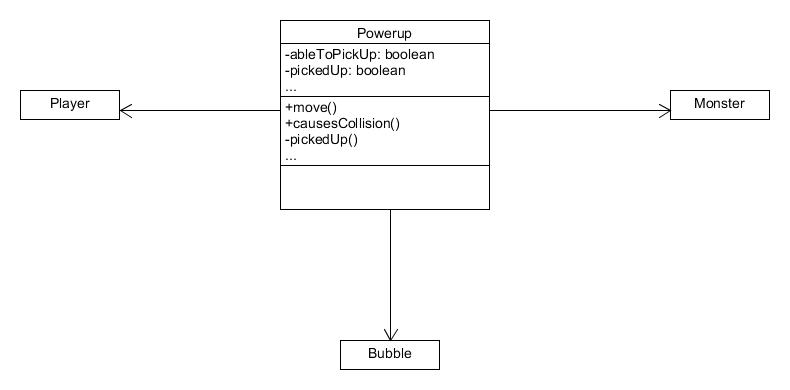
\includegraphics[width=100mm]{uml_powerups.jpg}\\[1cm]
The addition of a powerup is achieved by making a new class. This class is the instance of a powerup, as seen in the game. That is why it extends SpriteBase. 
\\\\
When a powerup is picked up, it triggers an effect. This effects for example Player, by increasing its speed. The relations in the UML above represent these effects.


\subsection{Multiple Lives: Responsibility Driven Design}

\subsubsection{Method}
\textit{Responsibility:} \\
\textit{Collaborations:}

\subsection{Multiple Lives: UML}

\subsection{A Score: Responsibility Driven Design}


\subsubsection{Method}
\textit{Responsibility:} \\
\textit{Collaborations:}

\subsection{A Score: UML}
